\section{Case studies}
The main purpose of developing efficient numerical method is to model real
world tsunami events and obtain accurate predictions in a timely manner. To demonstrate the applicability of the developed method, we consider two case studies. One is 2004 Indian Ocean tsunami caused by earthquakes in Sumatra island and the other is 2011 Japan tsunami caused by an earthquake in the coast of Tohuku. 

In order to model these events, it is important to obtain  accurate coastal
data, bathymetry distribution for the domain of interest, constructing the initial conditions for the forward wave modeling and setting up the boundary conditions. These are described in here.   
%\subsection{Case I: Indian Ocean tsunami modeling}
\label{sec:datasets}
 
\subsection{Coastal data}
Coastal data sets are needed to define the computational domain for these simulations. These are obtained from the Global Self-consistent, Hierarchical, High-resolution Shoreline (GSSHG  \cite{wessel2013gshhg}) a database provided by National Oceanographic and Atmospheric Administration (NOAA). 

\subsection{Computational mesh}
Triangular mesh aligned with complex coastlines is generated with an open-source mesh generation software tool GMSH. For the simulation in Indian Ocean, the mesh on the spherical surface is obtained from GMSH and is projected on 2D plane using a Mercator projection scheme. The generated mesh is shown in Fig (\ref{fig:indian_ocean_mesh}). This triangular mesh was provided to us by  the Alfred Wegner Institute, Germany.
For the simulation on world ocean, the mesh on the stereographic plane is obtained and projected on to the spherical surface. The generated mesh is show in Fig(\ref{fig:world_ocean_mesh}). This triangular mesh was provided to us by Bruno Seny. 
\begin{figure}[h!]
\begin{center}
\centering
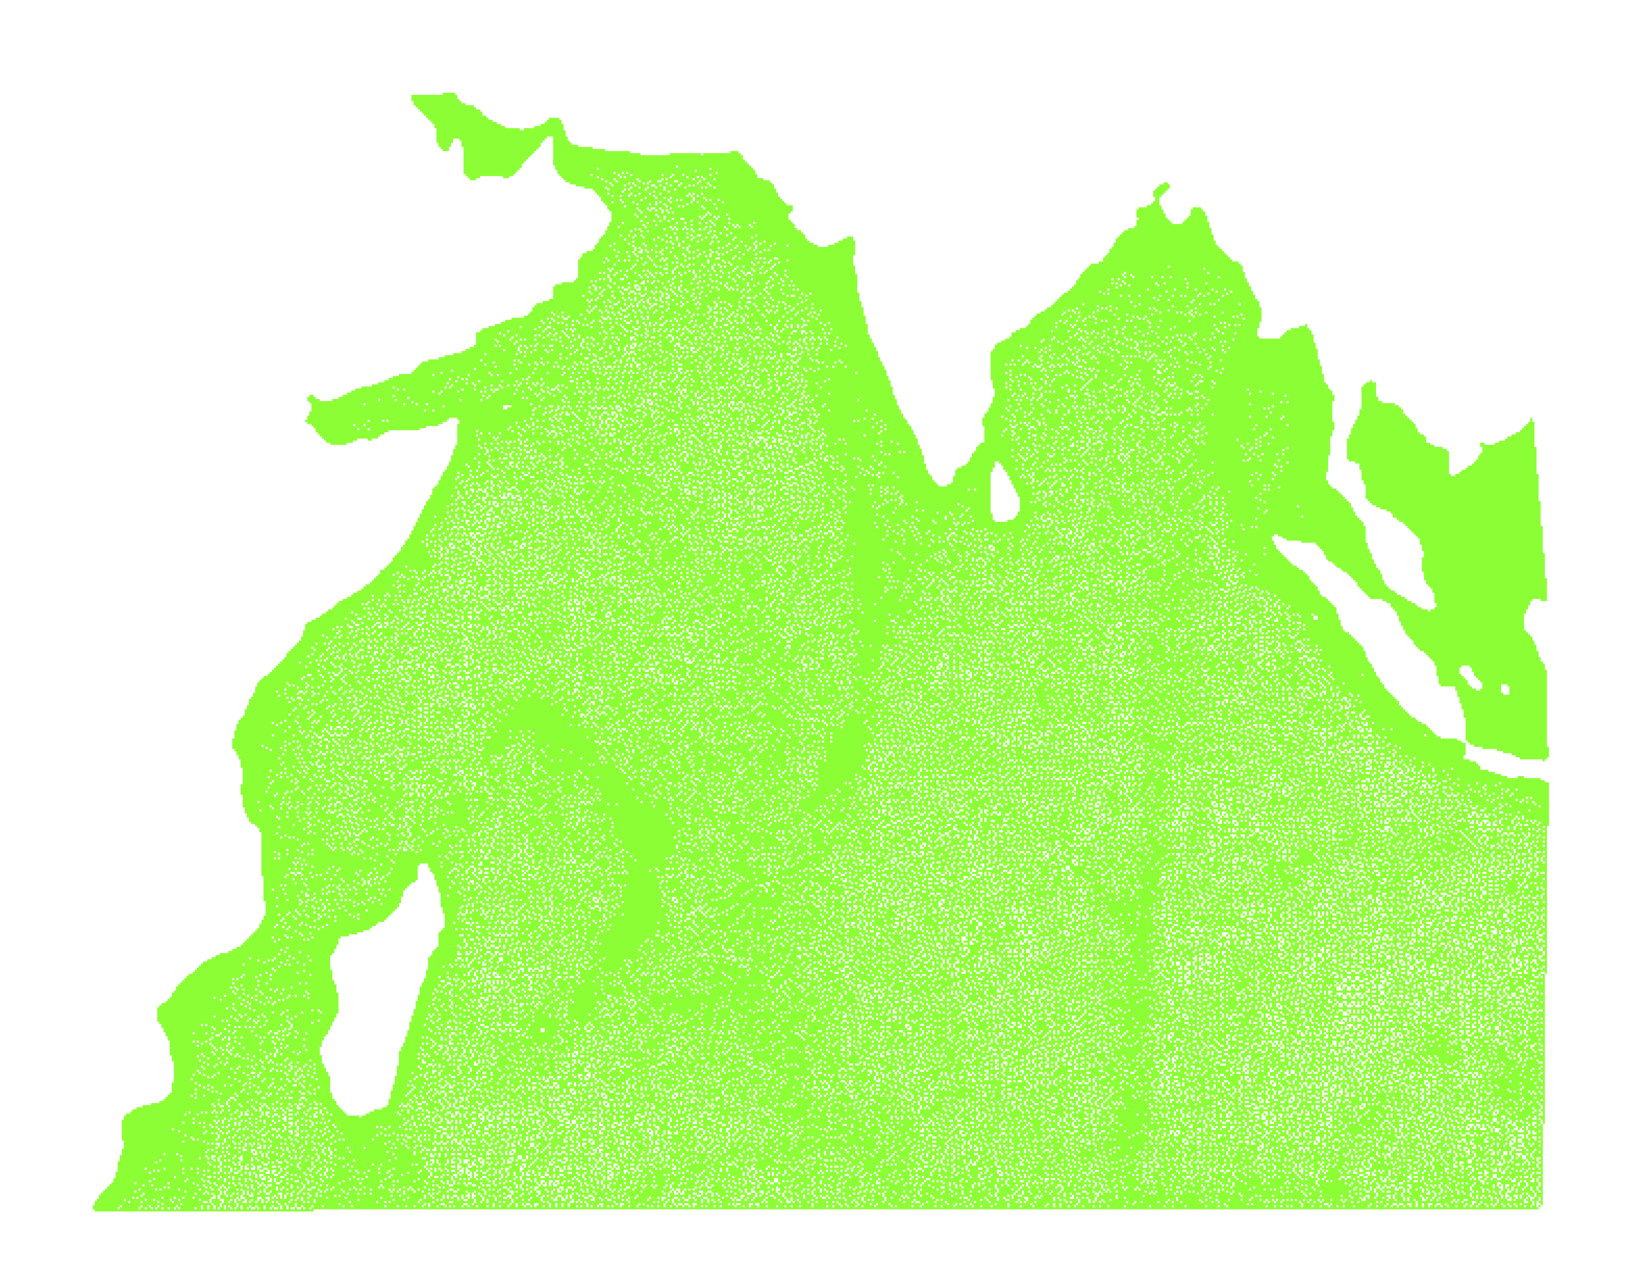
\includegraphics[trim=1.5cm 1cm 1.5cm 1.5cm,clip=true,width=0.5\linewidth]{./figures/IndianOcean.pdf}
\caption{\emph{Coastal aligned triangulation with 130,000 triangles of Indian Ocean.  Mesh and bathymetry distribution are provided by the Alfred Wegner Institute, Germany.}}
\label{fig:indian_ocean_mesh}
\end{center}
\end{figure}

\begin{figure}[h!]
\begin{center}
\centering
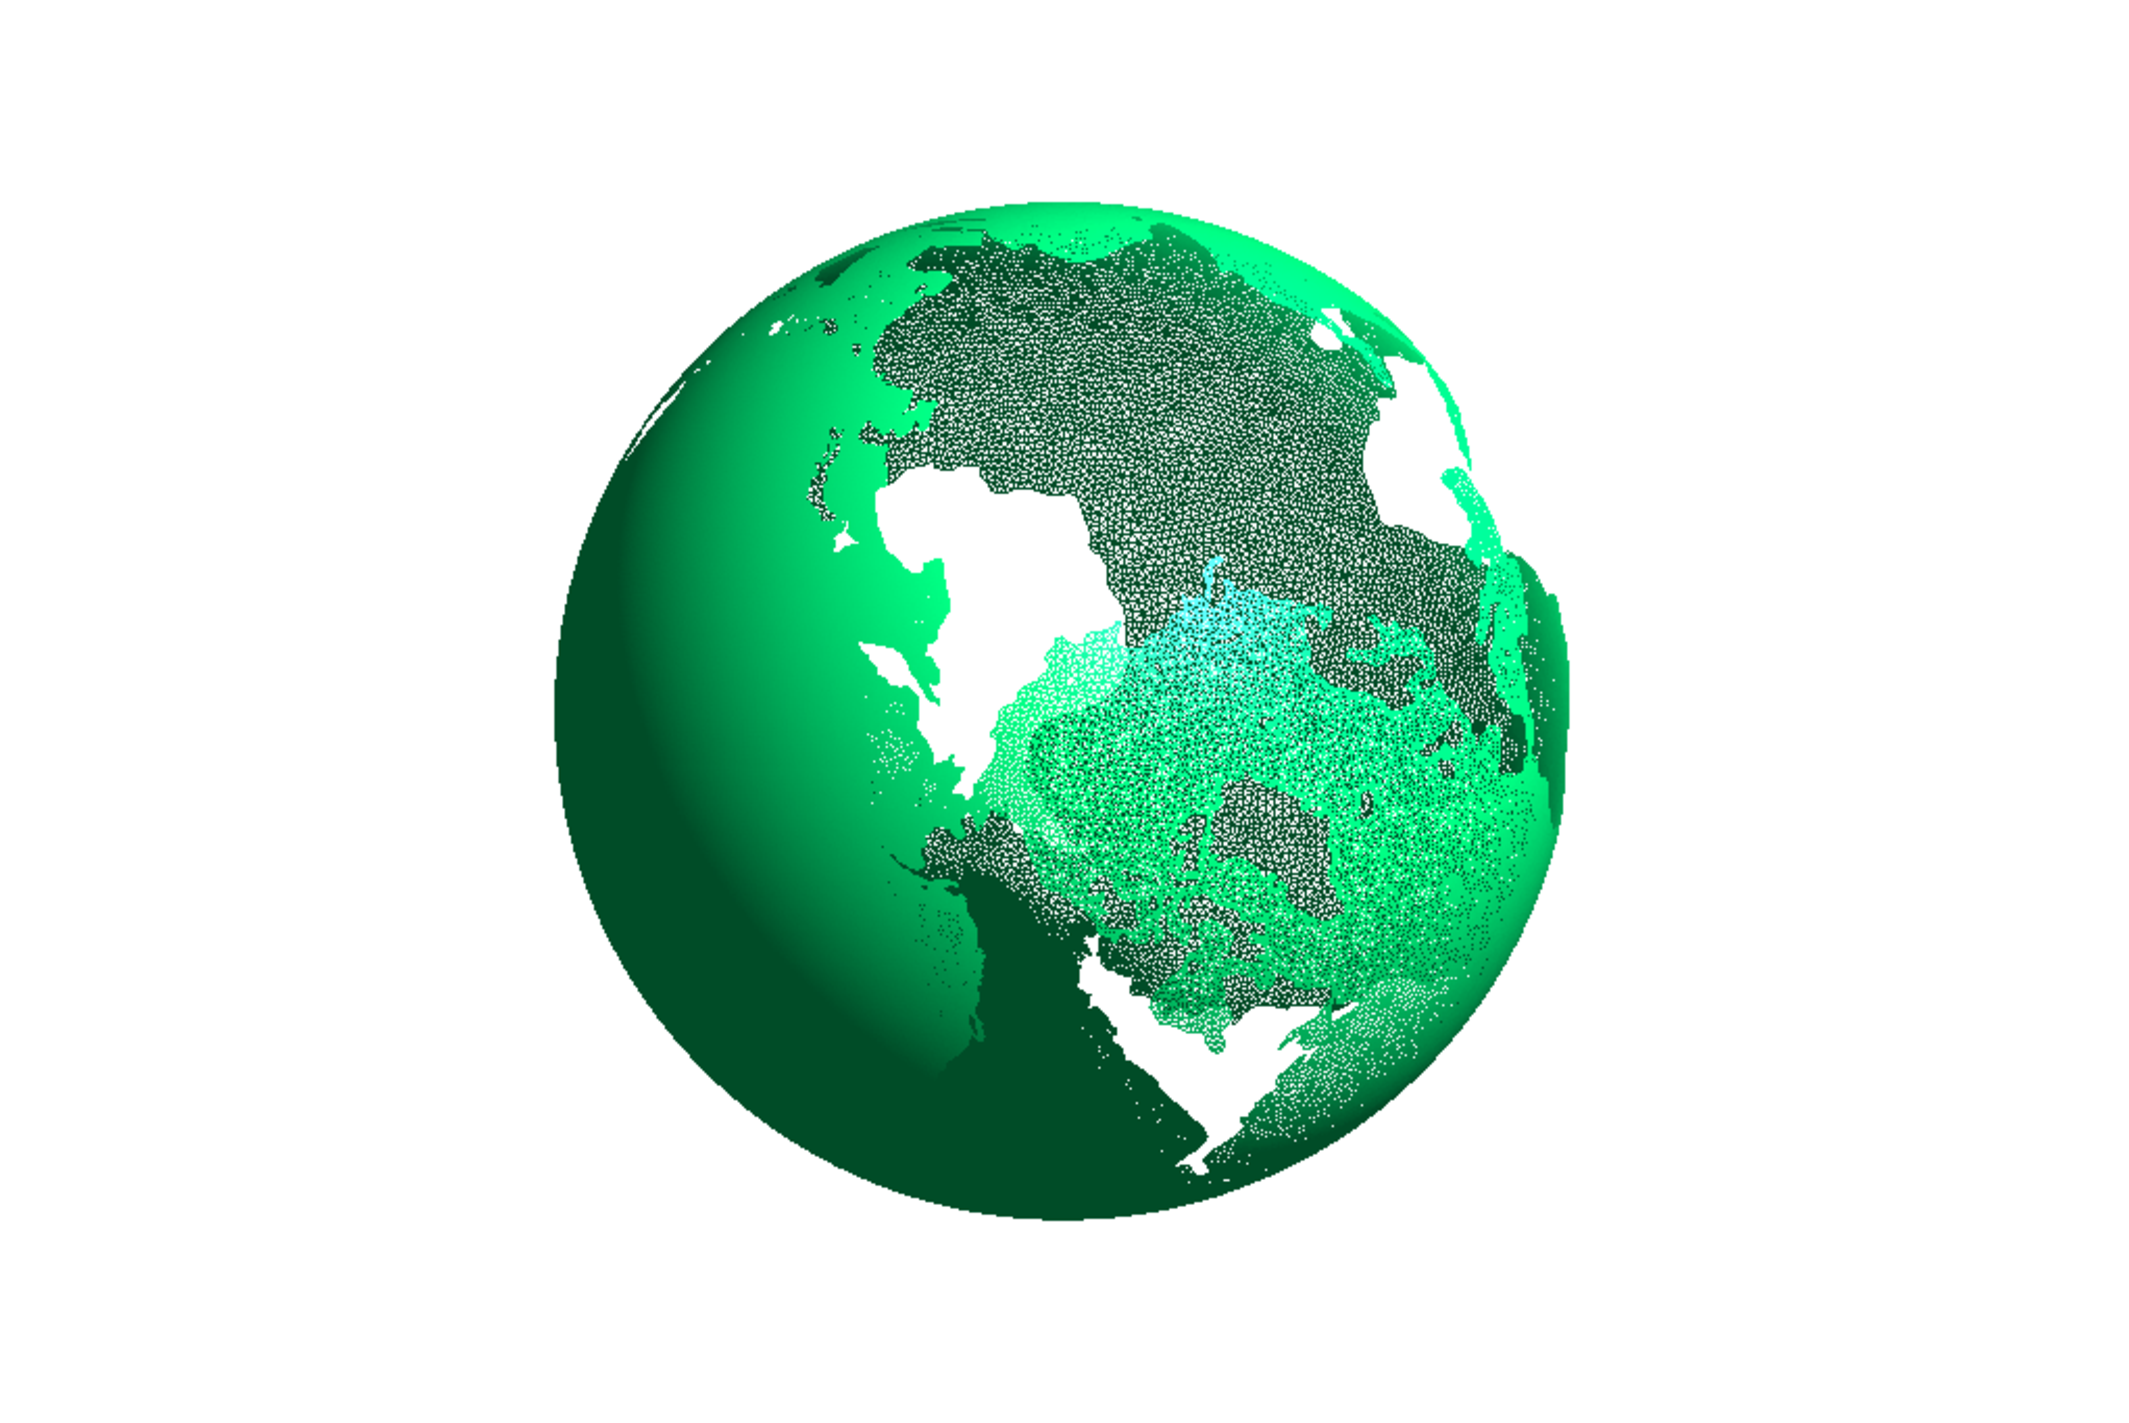
\includegraphics[trim=9cm 3cm 9cm 3cm,clip=true,width=0.5\linewidth]{./figures/globalOceanSphere.pdf}
\caption{\emph{Coastal aligned triangulation with 1,757,467 triangles of global
Ocean.}}
\label{fig:world_ocean_mesh}
\end{center}
\end{figure}

\subsection{Bathymetry distribution}
Accurate information on the ocean bed topography (or bathymetry) is crucial for tsunami simulations. This is because the speed of the tsunami waves is dictated by the water column height. Here, the ETOPO  \cite{amante2009etopo1} dataset from NOAA is used for the distribution of bathymetry. This information is also incorporated into mesh generation for defining mesh length scales.  The distribution of bathymetry in the Indian Ocean is shown in Fig (\ref{fig:indian_ocean_bathy}), in the world ocean is shown in Fig (\ref{fig:world_ocean_bathy}).
\begin{figure}[h!]
\begin{center}
\centering
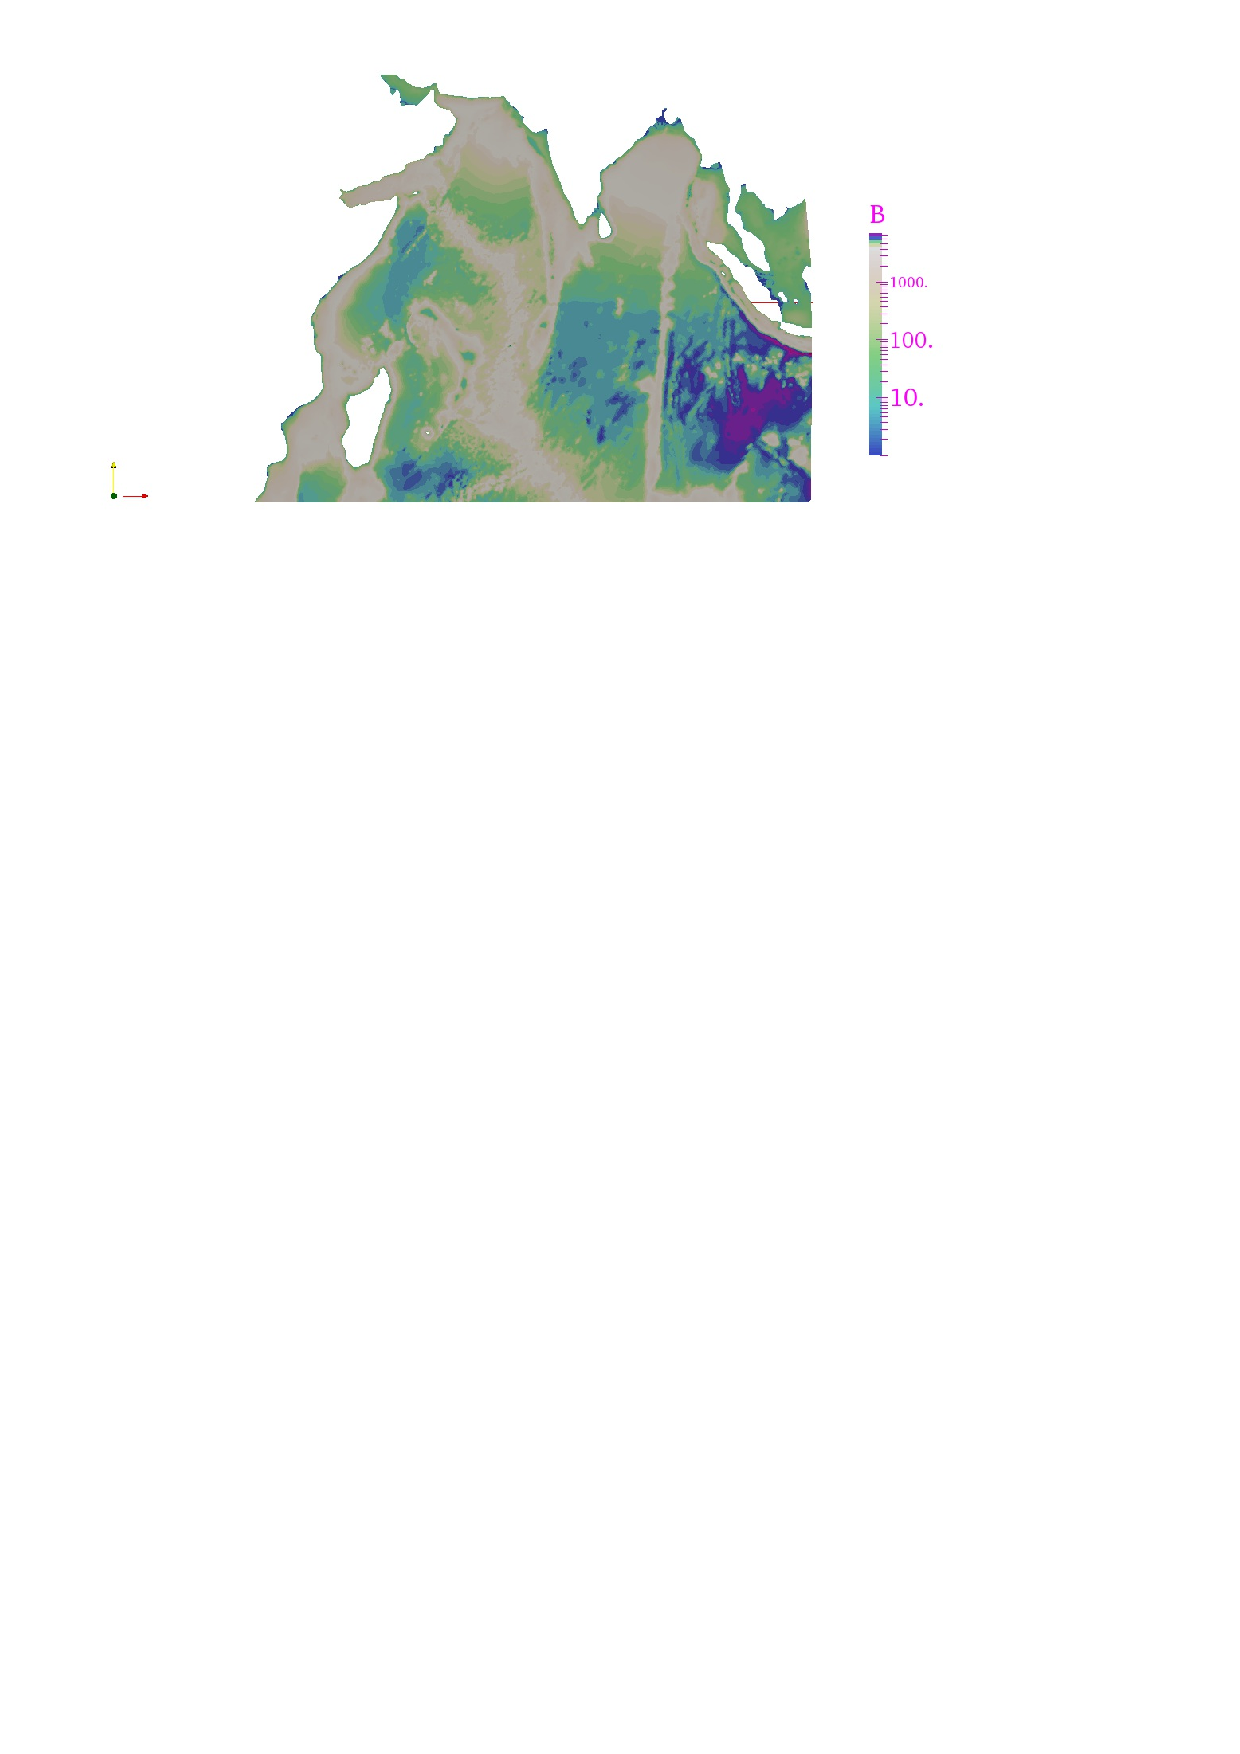
\includegraphics[trim=4.3cm 21.25cm 5.25cm 1.25cm,clip=true,width=0.5\linewidth]{./figures/IndianOceanBathy.pdf}
\caption{\emph{Bathymetry distribution (in meters) in Indian Ocean.}}
\label{fig:indian_ocean_bathy}
\end{center}
\end{figure}
\begin{figure}[h!]
\begin{center}
\centering
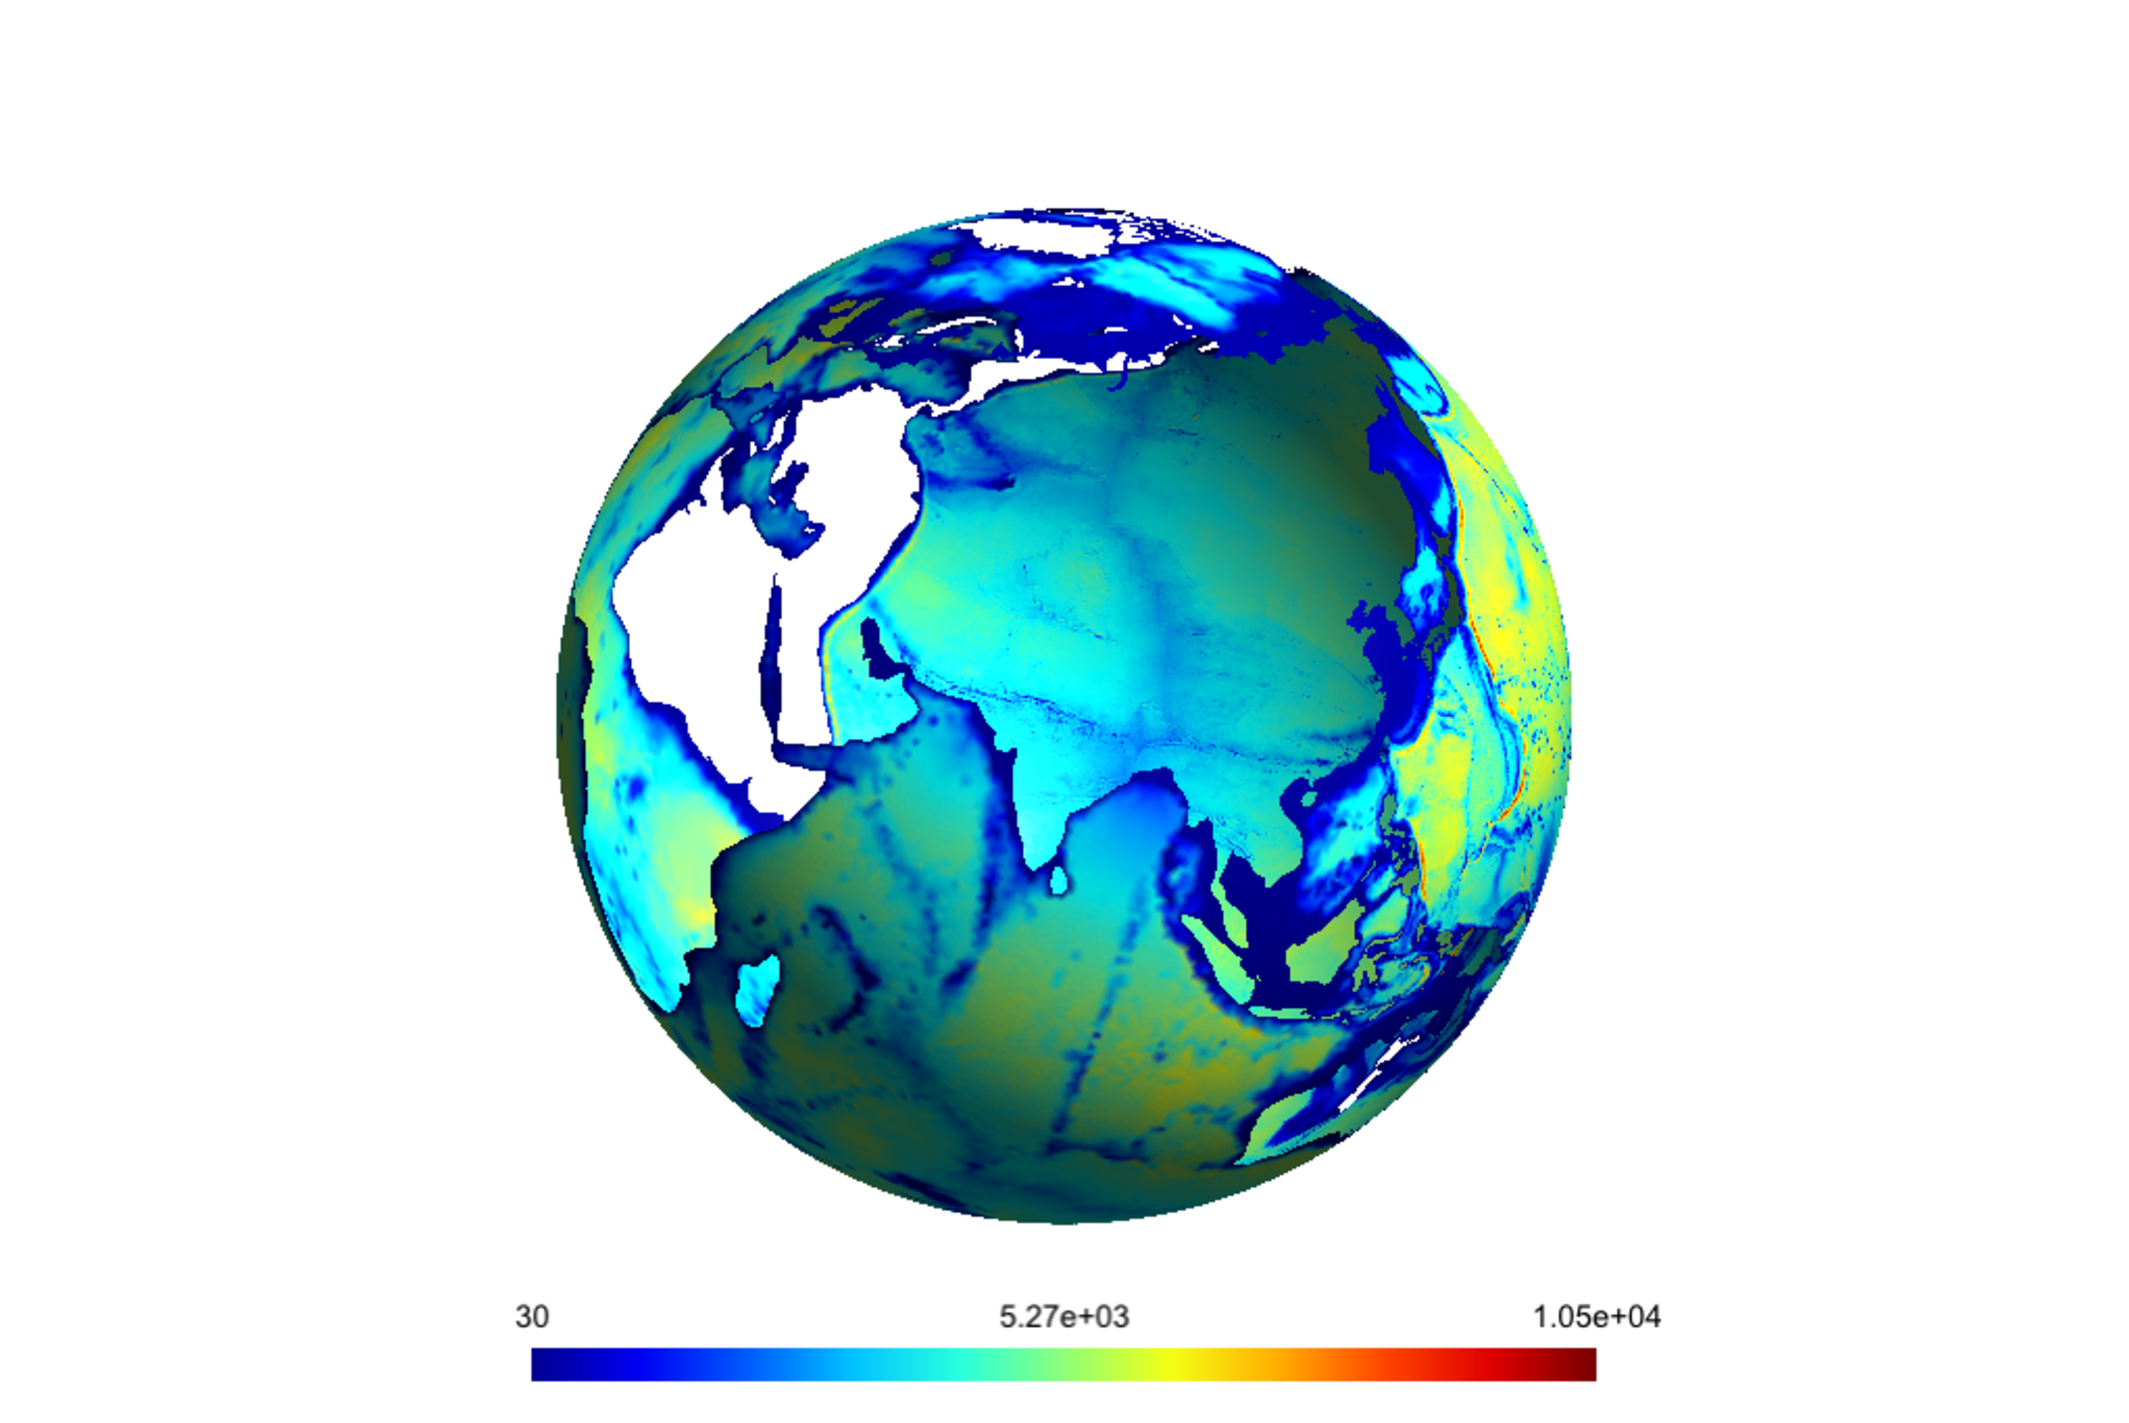
\includegraphics[trim=8cm 0cm 7cm 3cm,clip=true,width=0.5\linewidth]{./figures/globalOceanBathy.pdf}
\caption{\emph{Bathymetry distribution (in meters) in global ocean.}}
\label{fig:world_ocean_bathy}
\end{center}
\end{figure}

\subsection{Initial conditions}
Accurate representation of the initial wave generated after the earthquake event is required to simulate the wave propagation of the tsunami. In reality, the earthquake locations are not known and are estimated using several gauge recordings observed during the propagation of the wave (for an example,  see \cite{percival2011extraction}). For the validations, the initial surface displacement is estimated using the Okada model \cite{okada1992internal} and the earthquake data sets from United States Geological Services (USGS \cite{usgs}). The Okada model constructs the displacement of the seabed in the vertical direction, $Z$ at grid points ($X$, $Y$) using the fault plane parameters.

%The USGS earthquake data consists of five fault planes, given in Fig. (\ref{fig:indian_ocean_earth_quake}) \cite{ioualalen2007modeling}, that triggered Indian Ocean tsunami.  The vertical displacements due to each of these planes are obtained using Okada model and are aggregated to construct suitable initial conditions for forward wave propagation model. The constructed initial conditions are shown in Fig. (\ref{fig:indian_ocean_inc}). 

%\begin{figure}[h!]
%\begin{center}
%\centering
%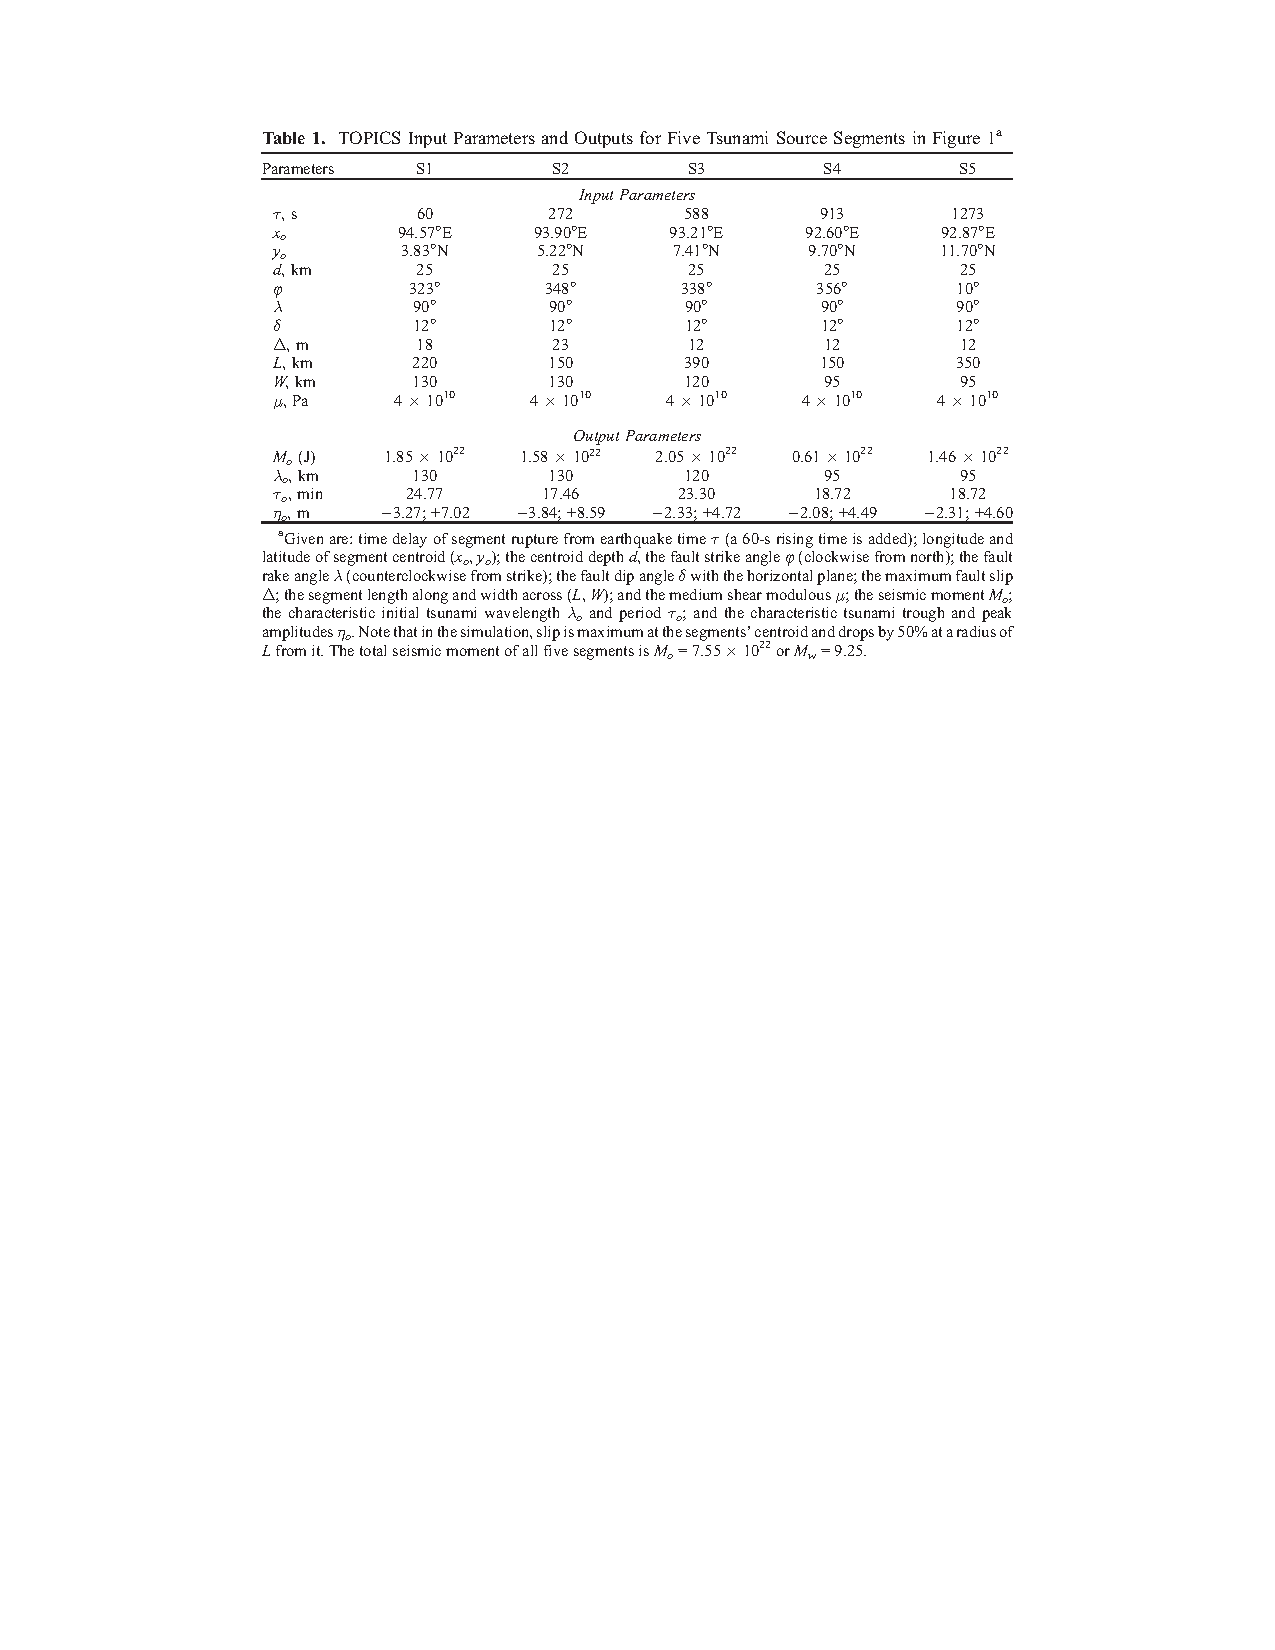
\includegraphics[trim=0cm 0cm 0cm 0cm,clip=true,width=\linewidth]{./figures/IndianOceanEarthQuake.pdf}
%\caption{\emph{Fault data of Sumatra earthquake. This  data is used as input for the Okada model to construct the initial displacement field of tsunami.}\cite{ioualalen2007modeling}}
%\label{fig:indian_ocean_earth_quake}
%\end{center}
%\end{figure}


\begin{figure}[h!]
\begin{center}
\centering
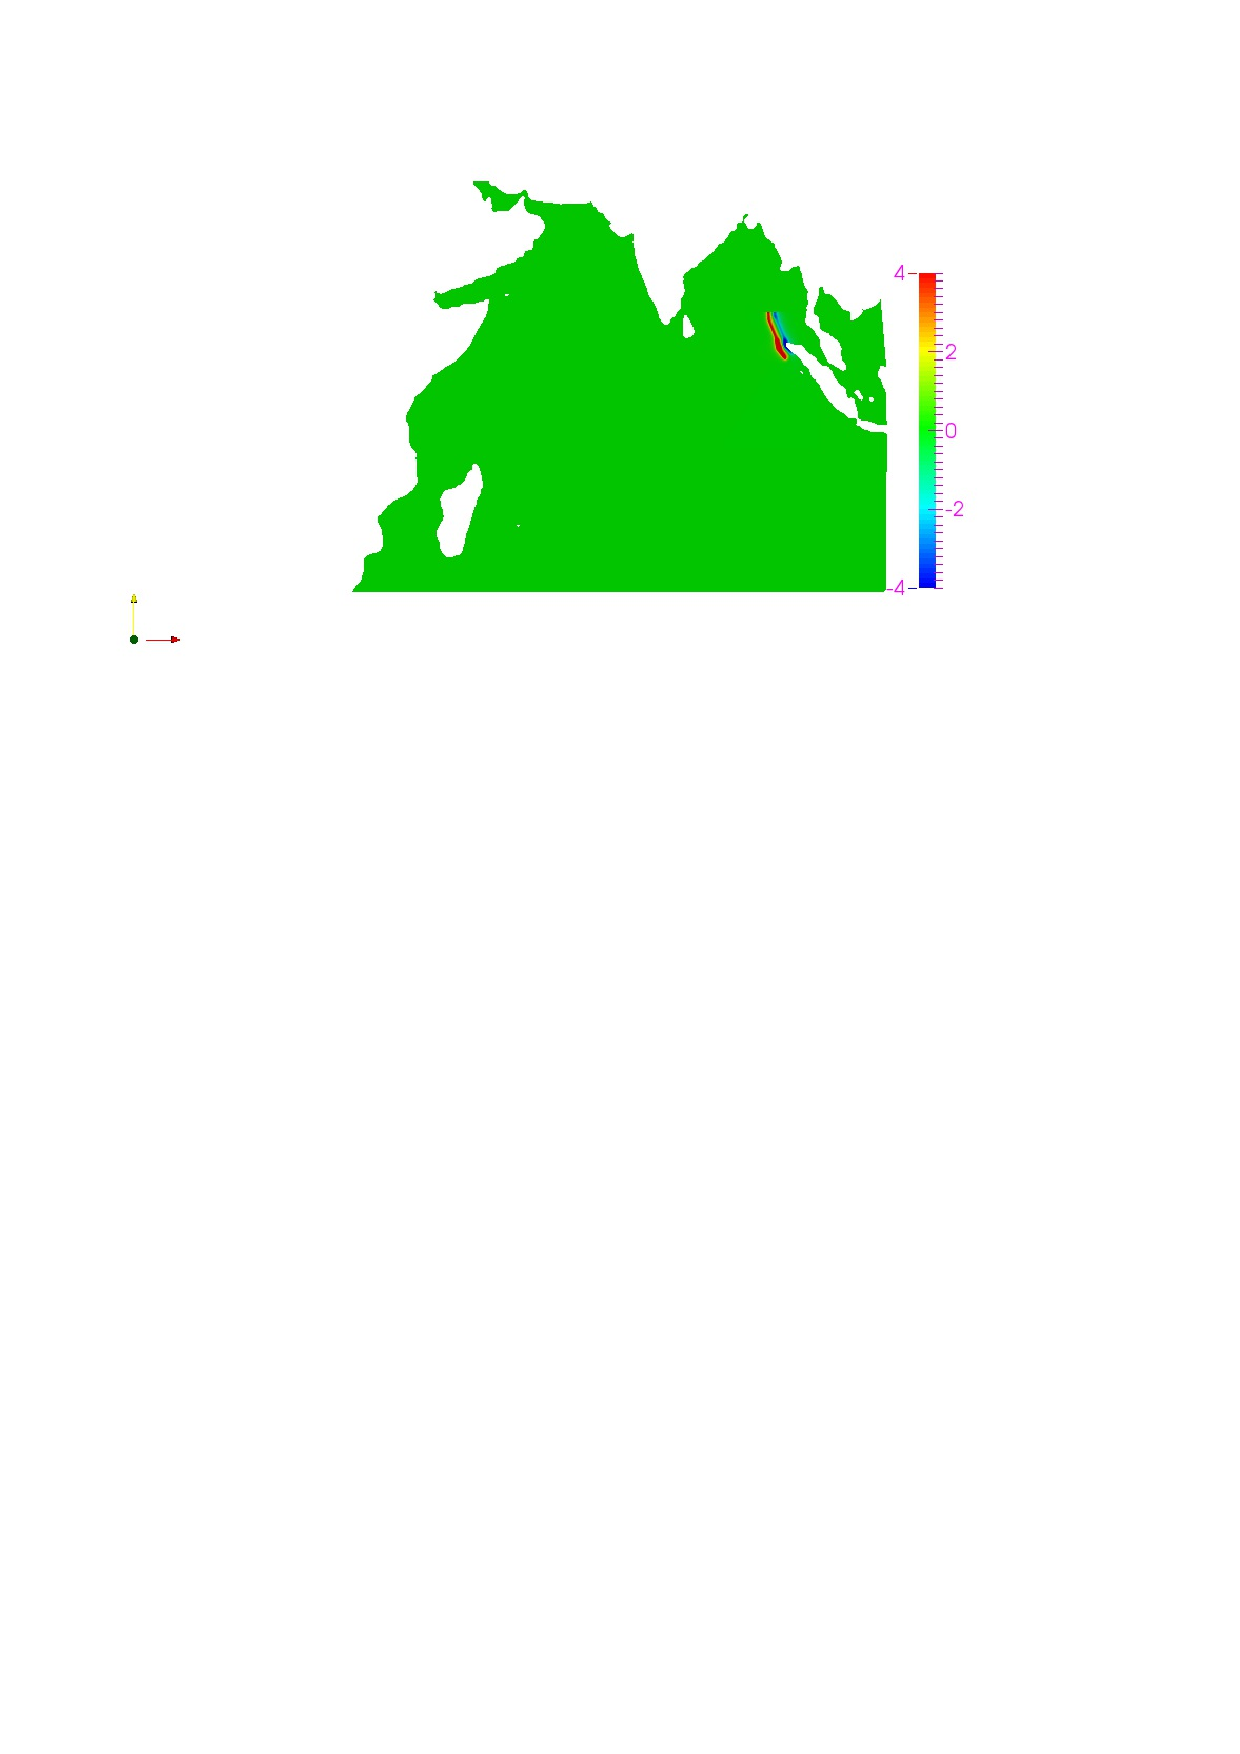
\includegraphics[trim=6cm 19.55cm 4.5cm 3cm,clip=true,width=0.5\linewidth]{./figures/IndianOceanINC.pdf}
\caption{\emph{Initial fluid displacement (in meters) from Okada model.}}
\label{fig:indian_ocean_inc}
\end{center}
\end{figure}

\subsection{Bottom friction}
Bottom friction force is parameterized by Ch\'ezy-Manning-Strickler formulation  \cite{gourgue2009flux} and is given by,
\begin{eqnarray}
\tau_{bx} &=& \frac{n^2 g}{h^{10/3}}\sqrt{(hu)^2+(hv)^2(}hu), \nonumber \\
\tau_{by} &=& \frac{n^2 g}{h^{10/3}}\sqrt{(hu)^2+(hv)^2}(hv)
\end{eqnarray}
here, $n$  is the Manning coefficient, an estimated roughness parameter of the ocean bed, is chosen to be $0.025~ s/m^{1/3}$, which is a typical value for sand. With the addition of the nonlinear forcing terms, the linear multi-rate time stepping is no longer stable. For the stability of the scheme the friction terms are integrated with implicit first order Euler method. The resulting scheme is an implicit-explicit time integration scheme. \begin{eqnarray}
\frac{dQ_H}{dt} &=& \mathcal{R}(Q_H) + S_b(Q_H),  \nonumber \\
Q_H^{n+1} -  \Delta t S_b\left(Q_{H} ^{n+1}\right) &=& Q_{H}^n + \sum_{i=0}^{2} \alpha_i\Delta t\mathcal{R}\left(Q_H ^{n-i}\right),
\end{eqnarray}
$S_b$ is the vector of bottom friction force, $Q_H ^n$ is the discrete solution at time step $n$, and  $\alpha_i$'s are coefficients of explicit multi-rate scheme. The above nonlinear system of equations is decoupled and point-wise. The exact solution of these equations can be obtained by solving a quadratic equation. However, the formula consists of a possibility of division with very small numbers, during the simulations. This leads to unstable rounding errors. Consequently, the nonlinear equations are linearized. %Consequently, these nonlinear equations are solved with Newton's method. The point-wise Jacobian matrix can be evaluated since the bottom friction is described by an analytical formula.

Adding the bottom friction is crucial near the shore where the fluid height is small. Fluid momentum builds up near shore and leads to large and unphysical velocities resulting in instabilities in the numerical solution. This instability is predominant for high order discretizations. Friction terms stabilize the flow in these regions and ensure the velocities to be bounded \cite{leveque2011tsunami}. 

\subsection{Boundary conditions}
Reflecting boundary conditions are imposed on the coastal boundary. However, the boundary conditions near the artificial boundary where the physical domain is truncated to a particular region of interest, is not straight forward. The artificial boundary reflects the outgoing waves into the physical domain. Thin sponge/absorbing layers are added near these boundaries \cite{modave2010parameters} to minimize these reflections. In these layers the numerical solution is nudged towards the exterior solution (zero in this context) by introducing a damping term in the PDE in these layers. We do not use the reflecting boundary conditions for the simulation in the world ocean since there are no unphysical boundaries. 

%The modified PDE in absorbing layers is given by,
%\begin{eqnarray}
%\frac{\partial \eta}{\partial t} + \frac{\partial F_1}{\partial x} + \frac{\partial G_1}{\partial y} &=& -(\sigma_x +\ \sigma_y) \eta, \nonumber \\
%\frac{\partial (hu)}{\partial t} +\ \frac{\partial F_2}{\partial x} + \frac{\partial G_2}{\partial y} &=& S_2 + \tau_{bx} - \sigma_x hu, \nonumber \\
%\frac{\partial (hv)}{\partial t} +\ \frac{\partial F_3}{\partial x} + \frac{\partial
%G_3}{\partial y} &=& S_3 + \tau_{by} - \sigma_y hv,
%\end{eqnarray}
%here, $\sigma_x$ and $\sigma_y$ are optimal damping coefficients derived for linear gravity waves. For one dimensional problem the coefficient $\sigma$ in the absorbing layer is given as,
%\begin{equation}
%\sigma(x) = \frac{\sqrt{gh}}{\delta} \frac{x}{\delta - x}, 
%\end{equation}
%here, $x$ is the distance from the outflow boundary and $\delta$ is the thickness of the absorbing layer. $\delta$ has to be sufficiently large in order to get significant damping of the outgoing waves in the absorbing layer. 

\subsection{Multi-rate time stepping}
At the beginning of the simulation, the elements are grouped into levels for the multi-rate time scheme, based on the elemental CFL condition. Fig (\ref{fig:indian_ocean_levels}), shows the distribution of the multi-rate levels for this simulation. Table (\ref{tab:pasidgLevels}), shows the percentage of elements grouped into each level.  From the figure it is clear that the elements near the shore are grouped into levels $3$ and $4$, that are the finest levels in the multi-rate scheme, whereas the elements in deep ocean are grouped in to levels $1$ and $2$, that are the coarsest levels. Only $2\%$ of the overall elements fall in to the finest level, resulting in $98\%$ of the elements requiring at most half of the computations when compared to a single rate scheme.

\begin{table}[h!]
\begin{center}
\begin{tabular}{crrrrr}
\hline
Level & \# elements & \% of elements & work per elem & \% of overall work\\ \hline
1 &  9960 &  7.63 & 1 & 2.60\\
2 & 60123 &  46.09 & 2 & 31.37\\
3 & 57441 & 44.04 & 4 & 59.94\\
4 &  2920 &  2.24 & 8 & 6.09\\\hline
\end{tabular}
\caption{\emph{Distribution of time stepping levels in multi-rate time integration
scheme.}}
\label{tab:pasidgLevels}
\end{center}
\end{table}
\begin{figure}[h!]
\begin{center}
%\centering
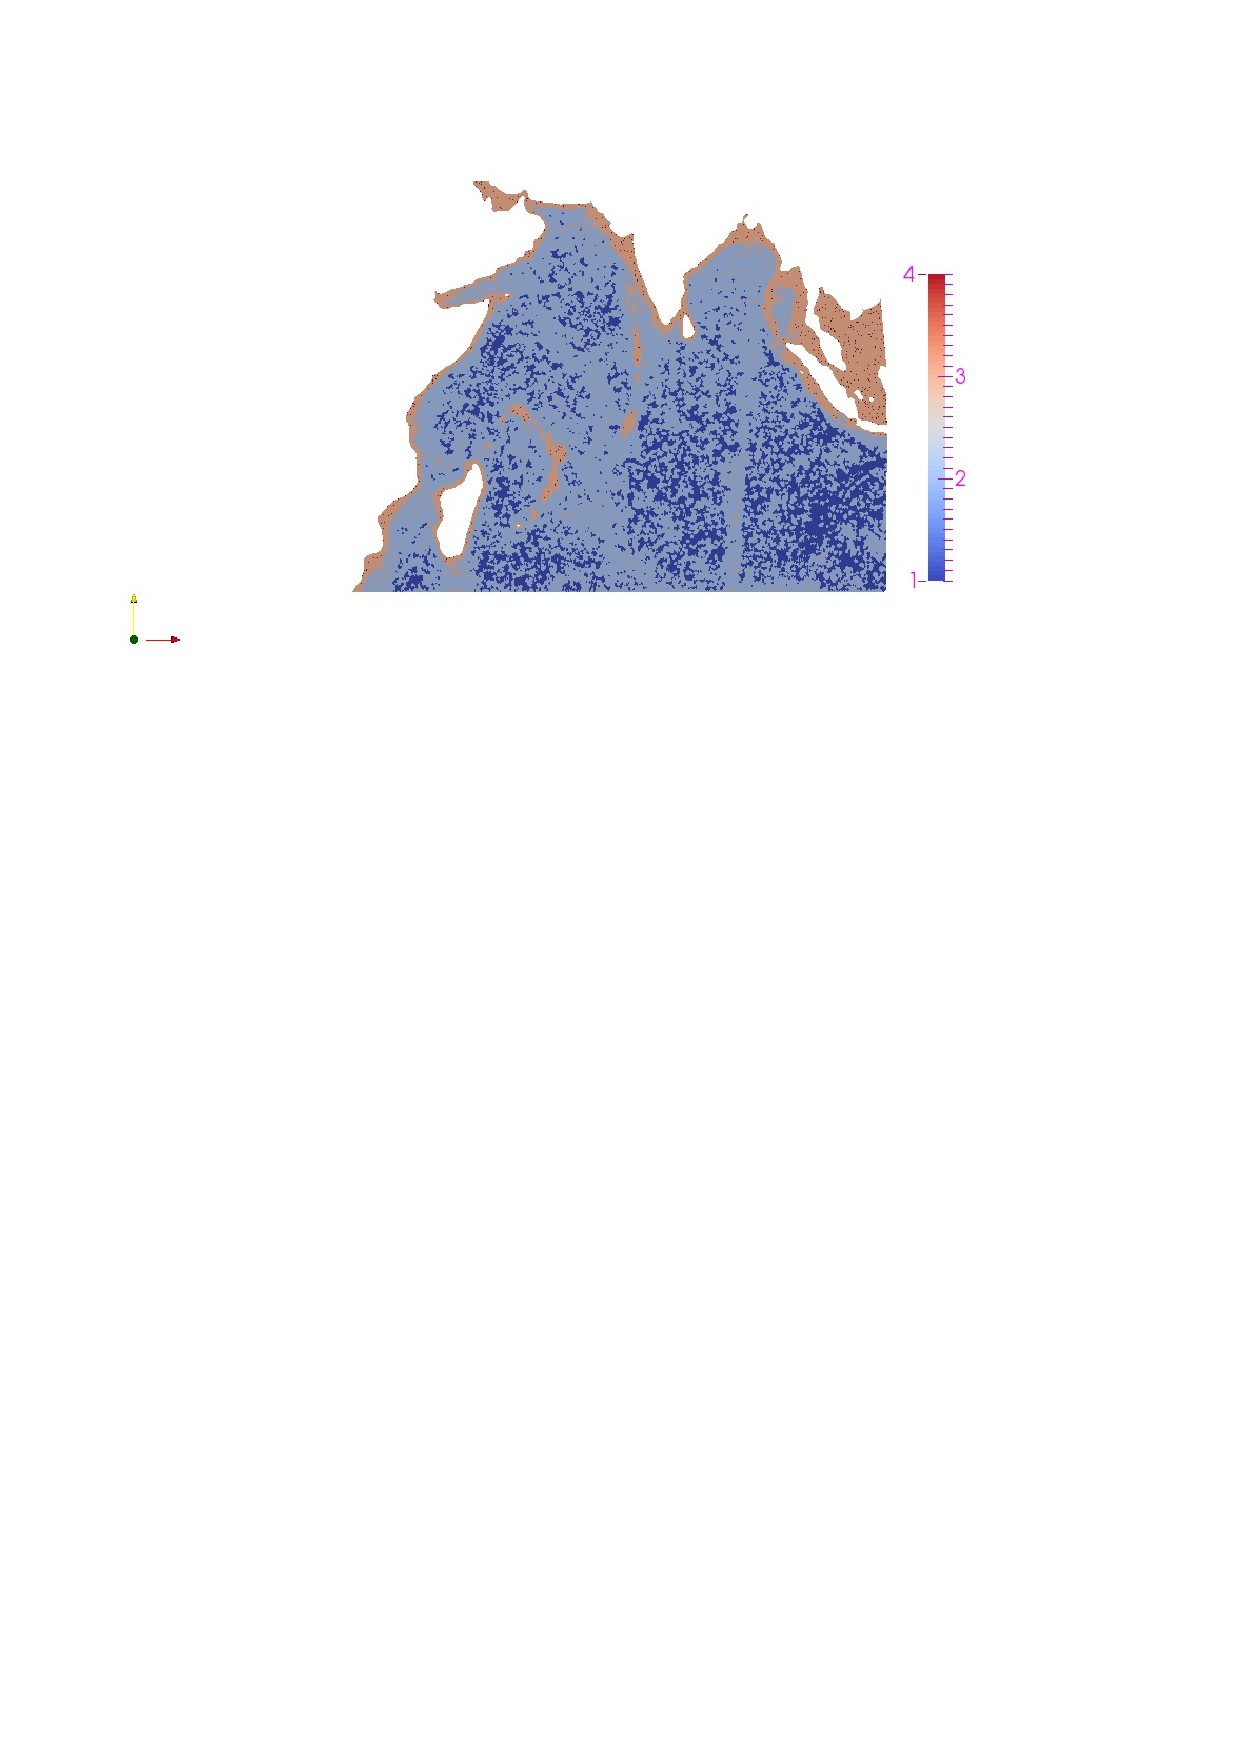
\includegraphics[trim=6cm 19.65cm 4.5cm 3.1cm,clip=true,width=0.5\linewidth]{./figures/IndianOceanLevels.pdf}
\caption{\emph{Distribution of  multi-rate levels for time stepping with
four levels.}}
\label{fig:indian_ocean_levels}
\end{center}
\end{figure}

